% content.tex
\tableofcontents
\newpage
\listoffigures
\newpage

% Include additional sections or chapters if needed
\chapter{Introduction}

Lithium-ion batteries are a type of battery that has become essential in our modern world. These batteries are lightweight and long-lasting, making them ideal for a wide range of applications such as smartphones, laptops, electric cars, and even power grids. The importance of lithium-ion batteries lies in their ability to store and provide energy efficiently, which helps reduce our reliance on fossil fuels and decrease carbon emissions.

Lithium-ion batteries offer high energy density, low self-discharge, and minimal maintenance, which further enhances their attractiveness for both consumer electronics and industrial uses. Electric vehicle's (EVs) provide the necessary power and efficiency to enable longer driving ranges and shorter charging times, driving the global shift towards greener transportation. Additionally, in renewable energy systems, lithium-ion batteries are critical for storing solar and wind energy, making it possible to supply electricity even when the sun isn't shining or the wind isn't blowing.

The versatility of lithium-ion batteries extends to their scalability and adaptability, making them suitable for small devices as well as large-scale energy storage systems. As technology continues to advance, the role of lithium-ion batteries will only become more prominent in powering our devices and moving toward a more sustainable future. Research and development efforts are ongoing to improve their performance, safety, and cost-effectiveness, ensuring that lithium-ion batteries remain at the forefront of energy storage solutions.

\begin{figure}[h!]
    \centering
    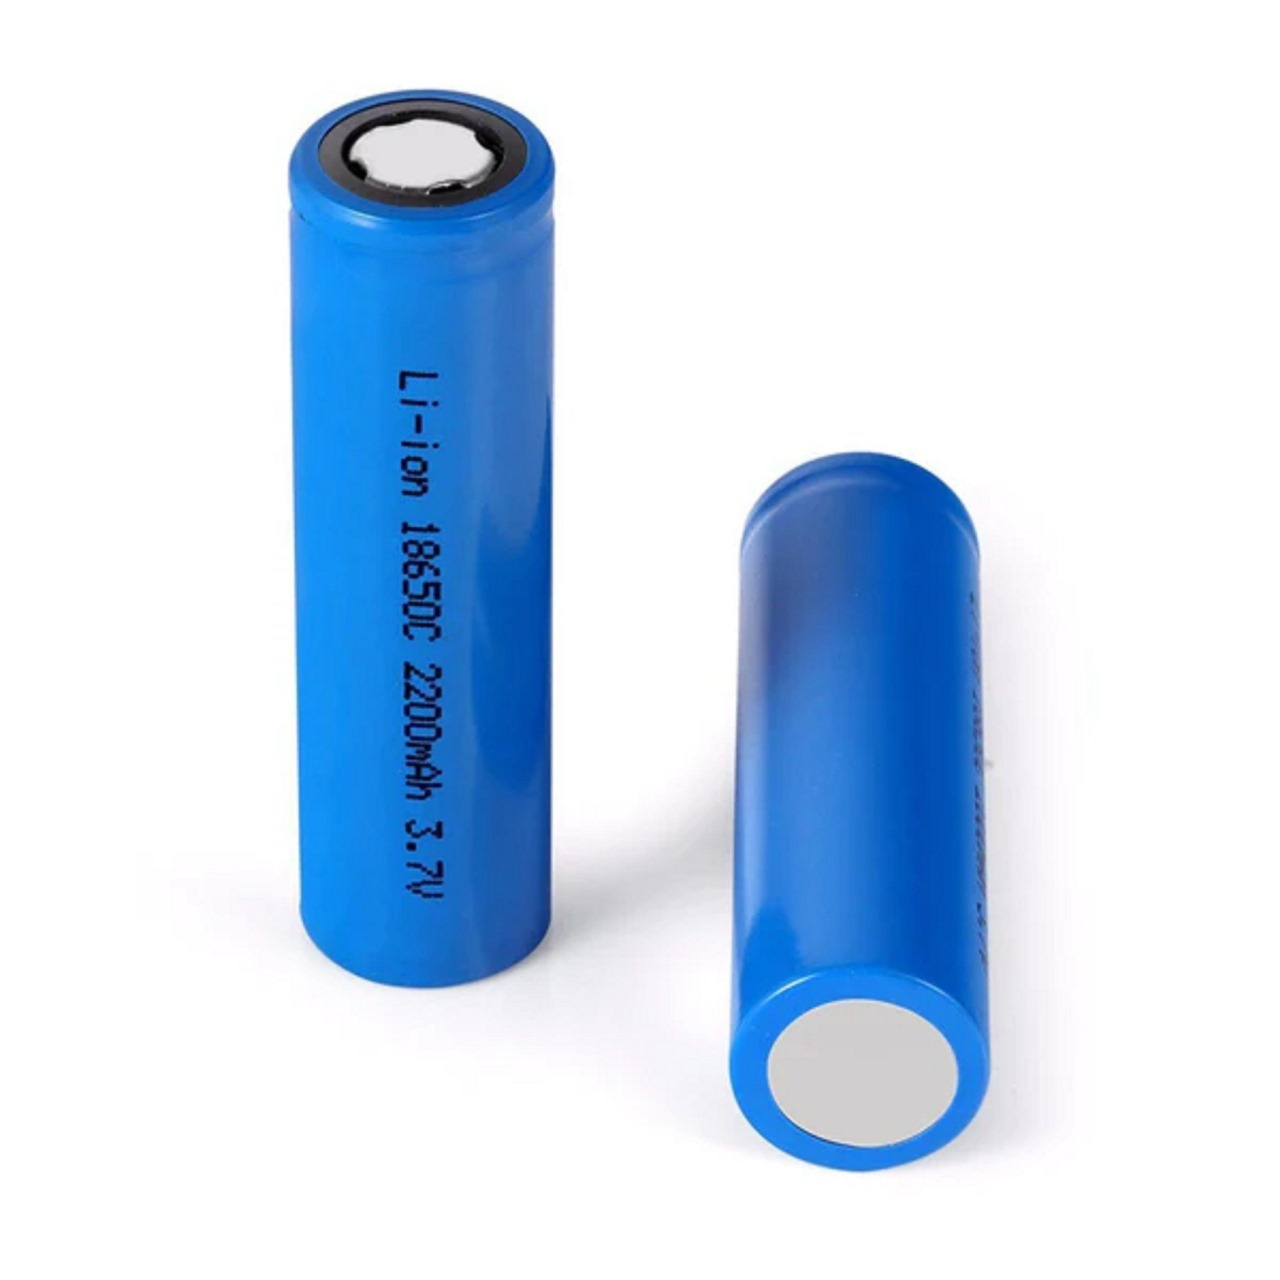
\includegraphics[width=0.5\textwidth]{importance_image.jpg} % Adjust the width as needed
    \caption{Li-ion Batteries }
    \label{fig:importance}
\end{figure}


\section{Importance of Estimation of SOH and RUL}
Understanding the state of health (SOH) and remaining useful life (RUL) of lithium-ion batteries is crucial for various reasons. These batteries play a significant role in powering a wide range of devices, from smartphones to electric vehicles. By accurately estimating their state of health, we can ensure their optimal performance and longevity. Additionally, knowing the remaining useful life of these batteries helps in planning for replacements and budgeting effectively. Without this information, there is a risk of unexpected failures, which can be costly and inconvenient.

Accurate estimations of SOH and RUL also enhance the safety of lithium-ion batteries. Over time, batteries can degrade and become prone to issues such as overheating, which can lead to safety hazards. By monitoring SOH and RUL, potential problems can be detected early, preventing accidents and ensuring user safety.

Furthermore, understanding SOH and RUL aids in the efficient recycling and repurposing of batteries. As the demand for lithium-ion batteries grows, so does the need for sustainable end-of-life management. Accurate assessments of battery health can determine whether a battery can be repurposed for less demanding applications or needs to be recycled. This reduces the environmental impact and conserves resources.

In industrial and commercial applications, such as grid storage and large-scale energy systems, precise SOH and RUL estimations can enhance the overall reliability and efficiency of energy management systems. Predictive maintenance enabled by these estimations ensures that energy systems operate smoothly, reducing downtime and maintenance costs.

Therefore, it is essential to prioritize the estimation of the state of health and remaining useful life of lithium-ion batteries to maximize efficiency, reliability, safety, and sustainability. This proactive approach not only extends the lifespan of batteries but also supports a more resilient and environmentally friendly energy infrastructure.

\begin{figure}[h!]
    \centering
    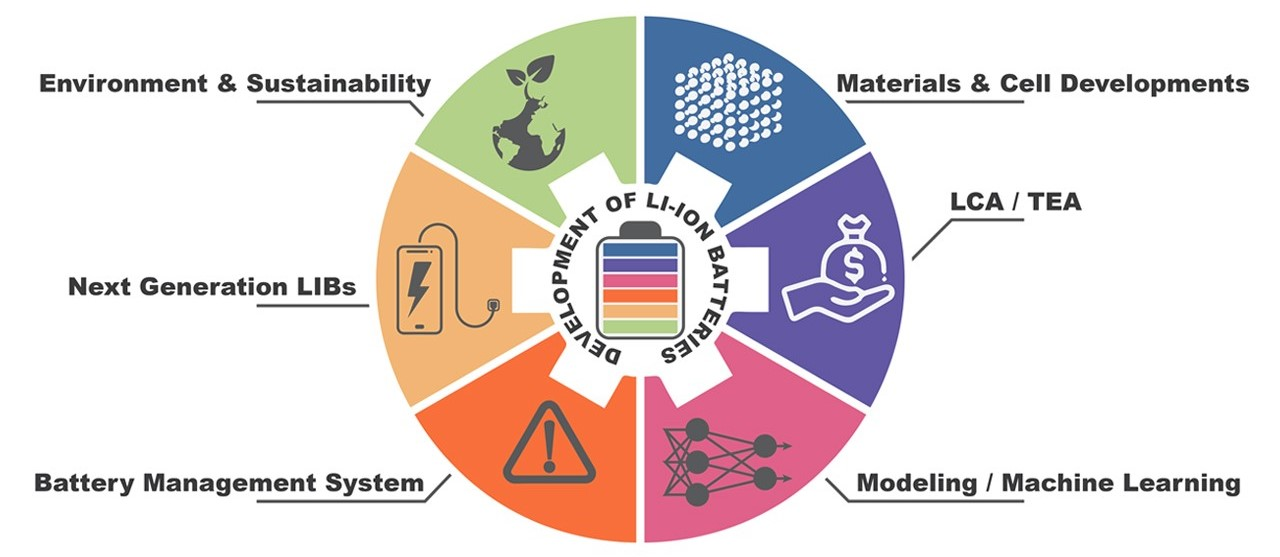
\includegraphics[width=0.95\textwidth]{graph.jpg} % Adjust the width as needed
    \caption{Trends \& Innovation in Li-ion batteries}
    \label{fig:another}
\end{figure}

\section{The Consequences of Inaccurate SOH and RUL Estimation}
\begin{figure}[h!]
    \centering
    \begin{minipage}[b]{0.45\textwidth}
        \centering
        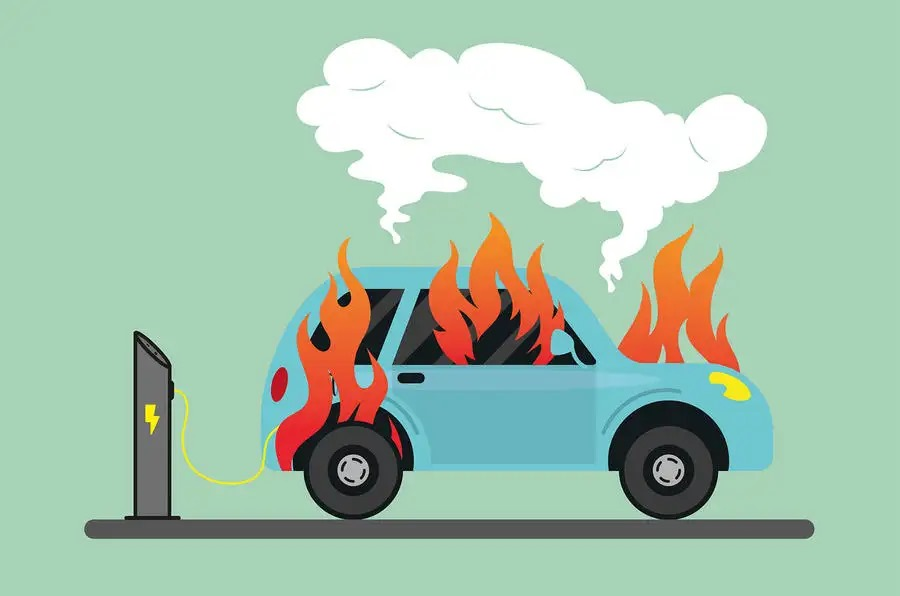
\includegraphics[width=1\textwidth, height=0.24\textheight]{consequences_image.jpg}
        \caption{EV Catching Fire}
        \label{fig:importance}
    \end{minipage}
    \hspace{0.05\textwidth}
    \begin{minipage}[b]{0.45\textwidth}
        \centering
        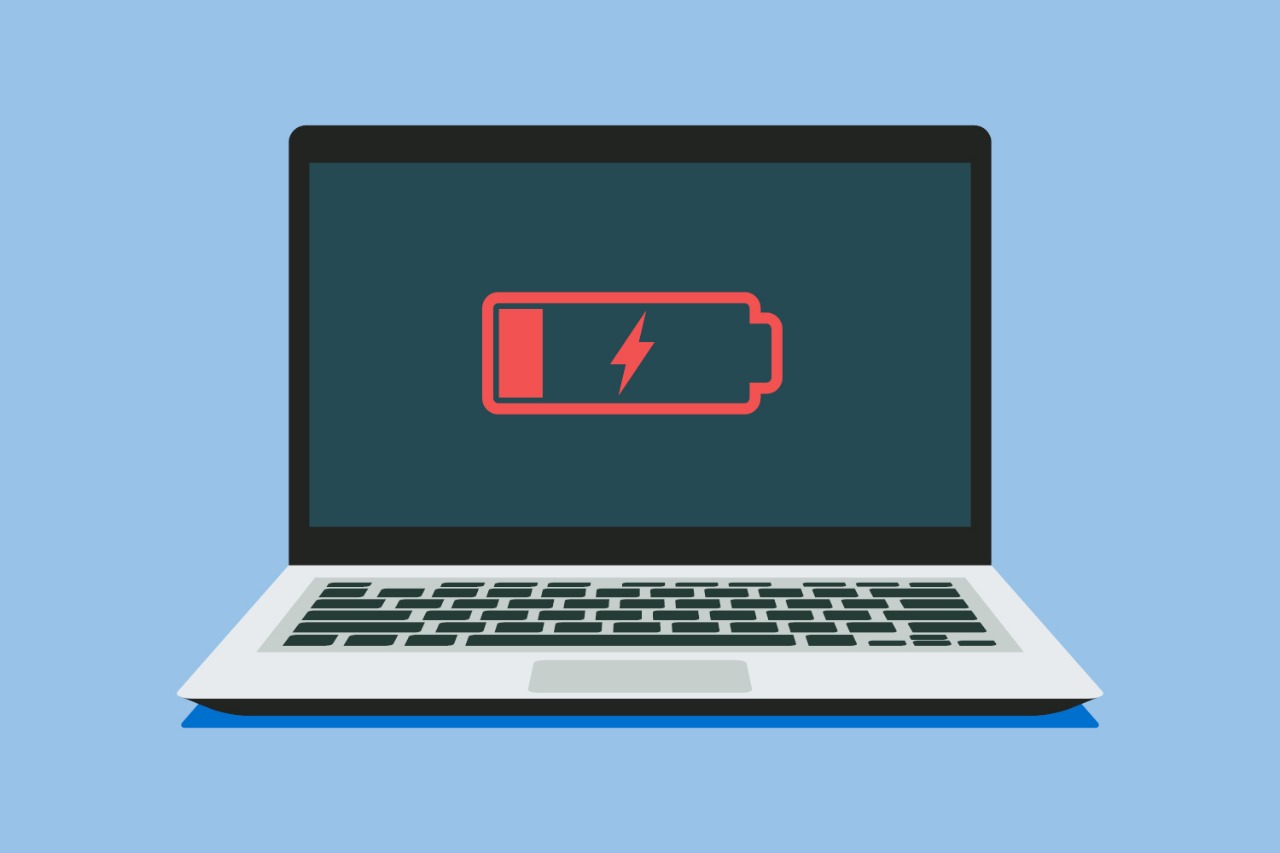
\includegraphics[width=1\textwidth, height=0.22\textheight]{consequences_image1.jpg}
        \caption{Laptop Battery Getting Degraded}
        \label{fig:another1}
    \end{minipage}
    \\
    \vspace{0.8cm} % Vertical space between rows of images
    \begin{minipage}[b]{0.45\textwidth}
        \centering
        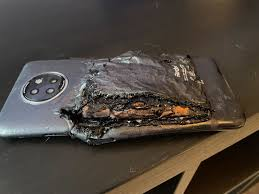
\includegraphics[width=\textwidth]{consequences_image2.jpg} % Adjust width to fit well
        \caption{Cell Phones Getting Exploded}
        \label{fig:another2}
    \end{minipage}
\end{figure}

Having an accurate understanding of the State of Health (SOH) and Remaining Useful Life (RUL) is crucial for managing battery systems. Failing to correctly estimate these parameters can lead to various negative consequences. For instance, inaccurate SOH and RUL estimation can pose safety risks such as battery overheating and explosions, which can endanger individuals and property. Moreover, not having a good grasp of SOH and RUL can result in reduced system performance, leading to unexpected power outages in electric vehicles or other critical applications. This not only inconveniences users but also has serious implications in terms of safety and reliability.

Inaccurate estimations can also disrupt supply chain management and logistics, particularly in industries relying on battery-powered equipment. For example, in electric vehicle fleets, unexpected battery failures can lead to significant operational downtimes and logistical challenges. This can affect delivery schedules, customer satisfaction, and overall business efficiency.

Additionally, inaccurate estimation of SOH and RUL may lead to increased maintenance costs, as batteries may be replaced prematurely, causing unnecessary expenses. Conversely, delaying battery replacement due to underestimated degradation can result in sudden failures, necessitating emergency repairs that are often more costly and disruptive.

Furthermore, this can have negative environmental impacts due to the premature disposal of batteries, contributing to electronic waste and pollution. Proper estimation allows for better planning of recycling and repurposing efforts, ensuring that batteries are utilized to their fullest potential before disposal.

Accurate SOH and RUL assessments also support the advancement of smart grid technologies and renewable energy integration. By reliably predicting battery performance and lifespan, energy storage systems can be more effectively managed, ensuring a stable energy supply from intermittent renewable sources like solar and wind.

\section{The Economic Benefits of Accurate RUL Prediction}
Accurately predicting the Remaining Useful Life (RUL) of batteries can result in significant cost savings and various economic benefits. By implementing precise RUL prediction techniques, companies can optimize their maintenance scheduling by replacing batteries only when necessary, thereby reducing unnecessary expenses. Moreover, improved system efficiency and performance can be achieved through timely battery replacements based on accurate RUL predictions. This not only saves costs but also ensures that systems operate at their peak performance levels.

Accurate RUL predictions can also enhance asset utilization. In industries such as transportation and logistics, knowing the exact lifespan of battery packs in electric vehicles or drones allows for better fleet management and deployment strategies. This maximizes the return on investment by ensuring each asset is fully utilized before replacement.

Furthermore, precise RUL estimations can improve the reliability and safety of critical systems. In sectors like healthcare, where battery-powered medical devices are used, ensuring that these devices function correctly without unexpected failures is paramount. Accurate RUL predictions help avoid sudden downtimes and maintain the integrity of these critical applications.

Additionally, extending the lifespan of batteries by replacing them at the right time can lead to long-term cost savings for businesses. This approach reduces the frequency of purchasing new batteries, thereby lowering capital expenditure. It also supports environmental sustainability by minimizing the disposal of batteries and reducing electronic waste.

Accurate RUL predictions can also facilitate better inventory management for battery manufacturers and suppliers. By understanding the lifespan of their products, manufacturers can better align production schedules with demand, thereby reducing excess inventory and associated holding costs.

\section{The Role of Machine Learning in Overcoming These Challenges}
Machine learning plays a crucial role in addressing challenges by providing a more advanced and data-driven approach compared to traditional methods. It offers more accurate estimations of State of Health (SOH) and Remaining Useful Life (RUL). By analyzing vast amounts of data, machine learning algorithms can identify patterns and trends that may go undetected by human-driven methods. This enables predictive maintenance strategies that can optimize performance, reduce downtime, and ultimately save costs.

Furthermore, machine learning models can continuously learn and improve over time as more data becomes available. This adaptability makes them particularly effective in dynamic environments where conditions and usage patterns may change frequently. For example, in electric vehicles, machine learning can be used to monitor battery health in real-time, providing insights that help in making informed decisions about maintenance and replacements.

Machine learning also facilitates the development of more sophisticated and reliable battery management systems (BMS). By integrating machine learning algorithms into BMS, it is possible to enhance the accuracy of SOH and RUL predictions, leading to better overall system performance. This integration supports the creation of more resilient and efficient energy storage solutions, which are essential for the advancement of renewable energy technologies and smart grid applications.

In conclusion, machine learning represents a powerful tool in overcoming the challenges associated with SOH and RUL estimation. Its ability to process and analyze large datasets, coupled with its continuous learning capabilities, makes it an invaluable asset in the pursuit of more accurate, reliable, and cost-effective battery management solutions.

\chapter{Battery Degradation Mechanisms}

Battery degradation is a natural process that occurs in various types of batteries over time, leading to a decrease in their performance and capacity. Different mechanisms contribute to battery degradation, such as lithium plating, electrolyte decomposition, and calendar aging. 

Lithium plating occurs when lithium ions unevenly accumulate on the surface of the anode, forming dendrites that can lead to short circuits and significantly shorten the battery's lifespan. Electrolyte decomposition occurs when the electrolyte breaks down, leading to the formation of gas bubbles, which can affect the battery's efficiency. Calendar aging, on the other hand, is the natural degradation of battery components over time due to chemical reactions that occur over time. 

In addition to these primary mechanisms, other degradation phenomena include the growth of the solid electrolyte interphase (SEI) layer and mechanical stresses. The SEI layer, which forms on the anode during initial charge cycles, can grow thicker over time, consuming active lithium and increasing internal resistance. Mechanical stresses, resulting from volume changes during charge and discharge cycles, can cause cracks and fractures in electrode materials, further degrading battery performance. 

\begin{figure}[h]
    \centering
    \begin{minipage}[b]{0.45\textwidth}
        \centering
        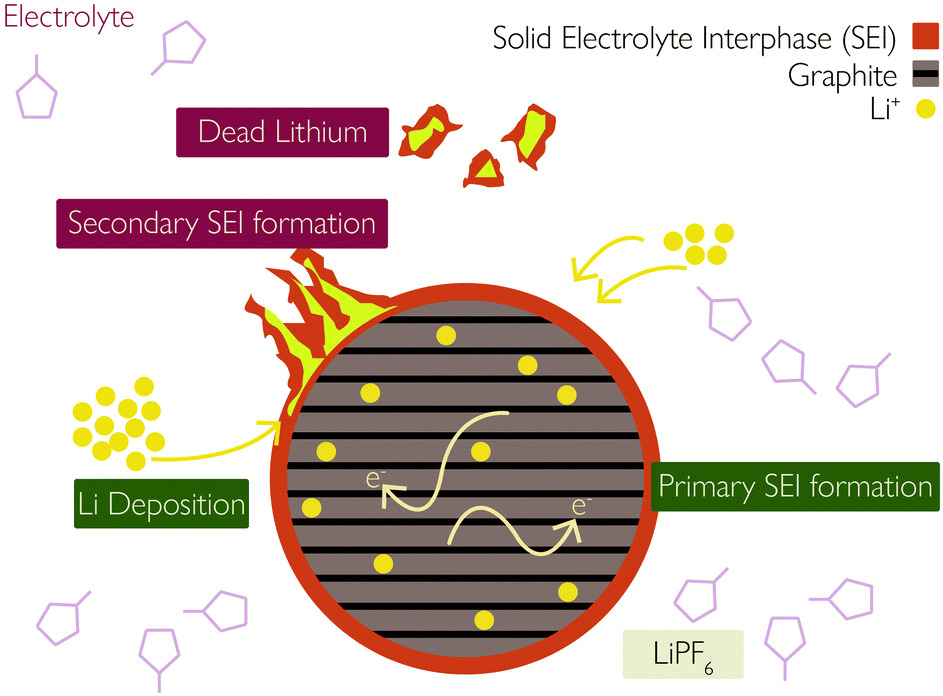
\includegraphics[width=\textwidth]{d1cp00359c-f2_hi-res.jpg}
        \caption{ Li-ion Battery Degradation }
        \label{fig:importance}
    \end{minipage}
    \hspace{0.05\textwidth} % Adjust the space between the figures as needed
    \begin{minipage}[b]{0.45\textwidth}
        \centering
        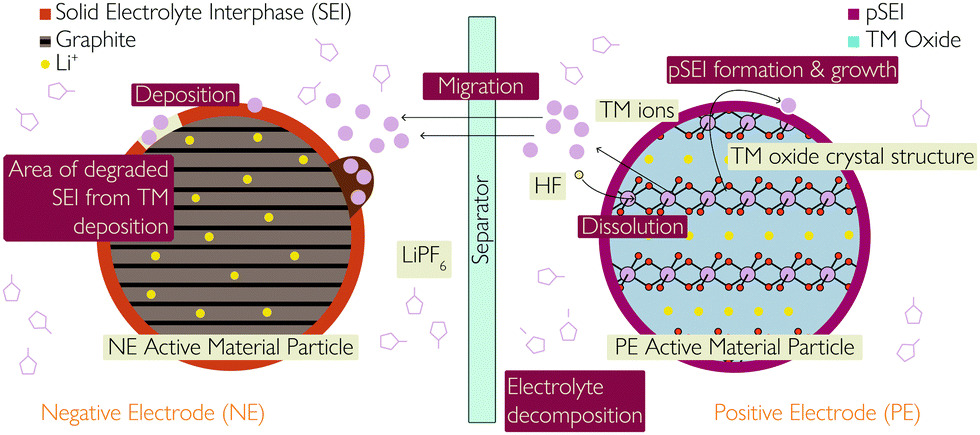
\includegraphics[width=\textwidth]{d1cp00359c-f4_hi-res.jpg} % Adjust width to fit well
        \caption{ Interaction between solid–electrolyte interphase (SEI) and lithium plating }
        \label{fig:another1}
    \end{minipage}
\end{figure}

Several factors influence battery degradation, including temperature, depth of discharge, and the number of charge/discharge cycles. High temperatures can accelerate the degradation process by enhancing chemical reactions that deteriorate battery materials. Deep discharge cycles and frequent charging can also contribute to reduced battery life by increasing the mechanical and chemical stresses on the battery components. Additionally, overcharging and rapid charging can exacerbate lithium plating and thermal runaway risks. 

Environmental conditions, such as humidity and exposure to air, can also impact battery degradation. Moisture can lead to the corrosion of battery terminals and the breakdown of electrolyte solutions, while oxygen exposure can oxidize electrode materials, further impairing battery function. 

Using relevant figures and diagrams can help illustrate these concepts and provide a better understanding of how battery degradation occurs. For example, diagrams showing the formation of dendrites during lithium plating, the breakdown of electrolytes, and the progression of SEI layer growth can visually represent these complex processes. Graphs illustrating the effects of temperature, depth of discharge, and charge/discharge cycles on battery capacity and performance over time can offer insights into how different factors accelerate degradation. 

\begin{figure}[h]
    \centering
    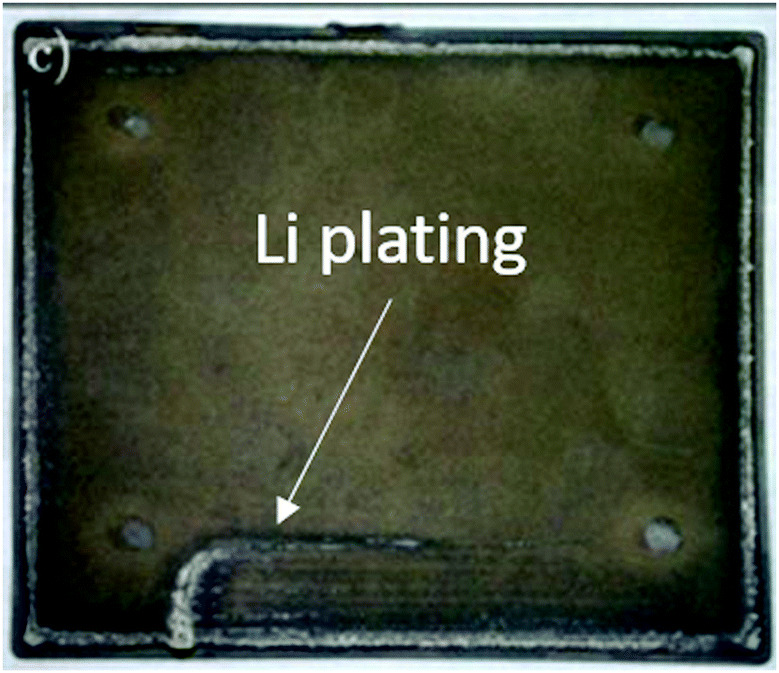
\includegraphics[width=0.4\textwidth]{d1cp00359c-f3_hi-res.jpg}
    \caption{Graphite electrode after extensive Li plating}
    \label{fig:graphite-electrode}
\end{figure}

To mitigate battery degradation, manufacturers are exploring advanced materials and technologies, such as solid-state electrolytes, which offer greater stability and safety. Battery management systems (BMS) are also being developed to monitor and control operating conditions, ensuring batteries are used within optimal parameters to extend their lifespan. Understanding these mechanisms and factors is crucial for developing strategies to improve battery longevity and performance, ultimately leading to more reliable and efficient energy storage solutions.


\chapter{TRADITIONAL METHODS FOR REMAINING USEFUL LIFE (RUL) PREDICTION}

Traditional methods for predicting the Remaining Useful Life (RUL) of machinery play a crucial role in maintenance planning and cost-saving efforts for various industries. These methods involve analyzing historical data, such as equipment performance, maintenance records, and environmental conditions, to estimate when a machine is likely to fail. By using techniques like statistical modeling, condition monitoring, and trend analysis, maintenance teams can proactively identify potential issues before they escalate, resulting in increased operational efficiency and reduced downtime. Implementing traditional RUL prediction methods can help organizations maximize the lifespan of their assets and make informed decisions about maintenance schedules and resource allocation.

Traditional methods for Remaining Useful Life (RUL) prediction often include calendar-based models and empirical models.

\section{Calendar-Based Models}

Calendar-based models predict RUL based on the elapsed time since the battery was put into service or since its last maintenance. These models assume a linear or exponential degradation of battery capacity over time. For instance, a simple calendar model might predict that a battery needs replacement after a certain number of years regardless of its actual usage.

\subsection{Limitations of Calendar-Based Models}

\begin{itemize}
    \item \textbf{Simplistic Assumptions:} These models often oversimplify battery degradation, assuming uniform degradation rates that may not reflect actual usage patterns or environmental conditions.
    \item \textbf{Lack of Adaptability:} They do not account for variations in usage, operational conditions, or different battery chemistries.
    \item \textbf{Limited Accuracy:} Predictions may be inaccurate if the actual degradation does not follow the assumed degradation pattern.
\end{itemize}

\section{Empirical Models}

Empirical models use historical data on battery performance and degradation obtained through testing or field observations. They typically involve fitting mathematical equation*s or statistical models to the data to predict RUL. Examples include models based on voltage trends, impedance measurements, or capacity fade over cycles.

\subsection{Limitations of Empirical Models}

\begin{itemize}
    \item \textbf{Data Dependency:} These models heavily rely on historical data, which may not always capture all relevant factors affecting battery degradation.
    \item \textbf{Generalization Issues:} They may not generalize well to new battery chemistries or operating conditions not represented in the training data.
    \item \textbf{Complexity in Calibration:} Calibration of empirical models can be complex and time-consuming, requiring extensive data collection and analysis.
\end{itemize}

\section{Physics-Based Models}

Physics-based models aim to simulate the underlying physical processes that contribute to battery degradation. These models incorporate fundamental electrochemical principles and equation*s to predict RUL based on factors such as electrode reactions, diffusion of ions, and thermal effects. They often require detailed knowledge of battery materials and complex numerical simulations.

\subsection{Limitations of Physics-Based Models}

\begin{itemize}
    \item \textbf{Complexity and Computational Cost:} Developing and calibrating physics-based models can be resource-intensive due to the complexity of electrochemical interactions and the need for accurate material parameters.
    \item \textbf{Assumptions and Simplifications:} Despite their basis in physical principles, these models still rely on simplifications and assumptions that may not fully capture all degradation mechanisms in real-world scenarios.
\end{itemize}

\section{Challenges with Traditional Methods}

\begin{itemize}
    \item \textbf{Limited Predictive Power:} Traditional methods often struggle to accurately predict RUL in dynamic and non-linear degradation scenarios. They may not capture sudden degradation events or changes in operating conditions effectively.
    \item \textbf{Dependency on Historical Data:} The accuracy of empirical and calendar-based models hinges on the availability and quality of historical data, which may not always be comprehensive or representative.
    \item \textbf{Adaptability to New Technologies:} As battery technologies evolve (e.g., new chemistries, electrode designs), traditional methods may struggle to adapt and provide accurate predictions without extensive recalibration or retraining.
\end{itemize}


\chapter{MACHINE LEARNING FOR RUL PREDICTION}

\begin{justifying}
Machine learning (ML) is a subset of artificial intelligence (AI) that involves the development of algorithms and statistical models that enable computers to perform specific tasks without explicit instructions. By learning from and making predictions based on data, ML algorithms can uncover patterns and relationships within complex datasets. This capability makes ML particularly suitable for tasks such as Remaining Useful Life (RUL) prediction, where traditional analytical methods might fall short due to the multifaceted and dynamic nature of battery degradation.

ML's adaptability and ability to process vast amounts of data from various sources enable more accurate and reliable predictions, thus enhancing maintenance strategies, optimizing performance, and reducing operational costs. This section explores various ML algorithms used for RUL prediction, including regression algorithms, time series forecasting algorithms, and deep learning algorithms, and discusses their advantages and disadvantages.
\end{justifying}

\section{Linear Regression}
\paragraph{Concept:}
Linear Regression is a commonly used statistical technique that models the relationship between a dependent variable and one or more independent variables by fitting a linear equation* to the observed data points.
\paragraph{Application to RUL Prediction:}
\begin{itemize}
    \item \textbf{Feature Selection:} Identify relevant features such as voltage, current, temperature, and usage patterns that influence battery degradation.
    \item \textbf{Model Training:} Fit a linear model to historical data to establish the relationship between these features and the battery's remaining capacity or performance metrics.
    \item \textbf{Prediction:} Use the trained model to predict the RUL based on current and future feature values.
\end{itemize}
\paragraph{Advantages:}
\begin{itemize}
    \item Simple and easy to implement.
    \item Provides interpretable results.
\end{itemize}
\paragraph{Disadvantages:}
\begin{itemize}
    \item Assumes a linear relationship between features and the target variable, which may not effectively capture complex degradation patterns.
\end{itemize}

\section{K-Nearest Neighbors (KNN)}
\paragraph{Concept:}
K-Nearest Neighbors is a non-parametric algorithm that predicts the value of a new data point based on the values of its k-nearest neighbors in the training set.
\paragraph{Application to RUL Prediction:}
\begin{itemize}
    \item \textbf{Feature Selection:} Identify relevant features such as voltage, current, temperature, and usage patterns that influence battery degradation.
    \item \textbf{Model Training:} Identify the k-nearest neighbors and average their RUL values to estimate the RUL of the new data point.
    \item \textbf{Prediction:} Use the trained KNN model to predict the RUL based on current and future feature values.
\end{itemize}
\paragraph{Advantages:}
\begin{itemize}
    \item Simple and intuitive approach.
    \item Can model non-linear relationships without assuming a specific form.
\end{itemize}
\paragraph{Disadvantages:}
\begin{itemize}
    \item Computationally intensive, especially with large datasets.
    \item Performance depends on choosing the appropriate k value and distance parameter.
\end{itemize}

\section{Support Vector Machines (SVM)}
\paragraph{Concept:}
Support Vector Machines are supervised learning models that can perform classification and regression tasks. SVM regression (SVR) tries to find a function that deviates from the true target values by a value no greater than a specified margin.
\paragraph{Application to RUL Prediction:}
\begin{itemize}
    \item \textbf{Feature Selection:} Identify features that influence battery degradation.
    \item \textbf{Model Training:} Train an SVR model to find the best-fit line (or hyperplane in higher dimensions) that stays within a specified margin of error.
    \item \textbf{Prediction:} Use the trained SVR model to predict the RUL based on current and future feature values.
\end{itemize}
\paragraph{Advantages:}
\begin{itemize}
    \item Effective in high-dimensional spaces and against overfitting in low-dimensional spaces.
    \item Flexible through the use of different kernel functions.
\end{itemize}
\paragraph{Disadvantages:}
\begin{itemize}
    \item Computationally intensive and memory demanding, especially with large datasets.
    \item Requires careful tuning of hyperparameters (e.g., margin width, kernel type).
\end{itemize}

\section{Decision Tree}
\paragraph{Concept:}
Decision Trees are a type of supervised learning algorithm that splits the data into subsets based on the value of input features, creating a tree-like model of decisions.
\paragraph{Application to RUL Prediction:}
\begin{itemize}
    \item \textbf{Feature Selection:} Identify features influencing battery degradation.
    \item \textbf{Model Training:} Build a tree by recursively splitting the training data based on feature values to minimize prediction error at each node.
    \item \textbf{Prediction:} Traverse the tree using the eigenvalues of new data points to arrive at a leaf that gives the estimated RUL.
\end{itemize}
\paragraph{Advantages:}
\begin{itemize}
    \item Easy to understand and interpret.
    \item Handles both numerical and categorical data.
\end{itemize}
\paragraph{Disadvantages:}
\begin{itemize}
    \item Prone to overfitting, especially with deep trees.
    \item Sensitive to small variations in the data.
\end{itemize}

\section{Random Forest}
\paragraph{Concept:}
Random Forest is an ensemble learning method that constructs multiple decision trees during training and outputs the mean prediction of the individual trees.
\paragraph{Application to RUL Prediction:}
\begin{itemize}
    \item \textbf{Feature Selection:} Identify relevant features influencing battery degradation.
    \item \textbf{Model Training:} Build multiple decision trees using different subsets of the training data and features. Each tree provides a prediction, and the final RUL prediction is the average of these individual predictions.
    \item \textbf{Prediction:} For a new data point, run it through each tree in the forest and average the results to obtain the final RUL prediction.
\end{itemize}
\paragraph{Advantages:}
\begin{itemize}
    \item High prediction accuracy due to ensemble averaging.
    \item Robust to overfitting and can handle large datasets well.
\end{itemize}
\paragraph{Disadvantages:}
\begin{itemize}
    \item Complex and difficult to interpret compared to single decision trees.
    \item Requires significant computational resources for training.
\end{itemize}


\chapter{Battery Data Collection and Pre-processing}

\begin{justifying}
Data plays an important role in machine learning (ML) models, especially for tasks such as predicting battery life (RUL). The quality, quantity, and accuracy of data directly affect the accuracy and reliability of the forecast. Important aspects include:

\begin{itemize}
    \item \textbf{Prediction Accuracy:} Good information ensures that the ML model can learn meaningful patterns and relationships to accurately predict RUL.
    \item \textbf{Generalization:} Diverse datasets help generalize learning models to unseen data, thus increasing their robustness and reliability in practical use.
    \item \textbf{Feature Selection and Engineering:} Identifying and processing relevant features (such as voltage, current, temperature) is crucial for model performance.
\end{itemize}

The Hawaii Natural Energy Institute dataset contains data for 14 NMC-LCO 18650 cells, each with a capacity of 2.8 Ah. These batteries were cycled over 1000 times at 25°C using a CC-CV (Constant Current-Constant Voltage) charge rate of C/2 and a discharge rate of 1.5 C. The dataset provides insights into various operational parameters recorded during these cycles, which are crucial for predicting the RUL of batteries.
\end{justifying}

\begin{figure}[h!]
    \centering
    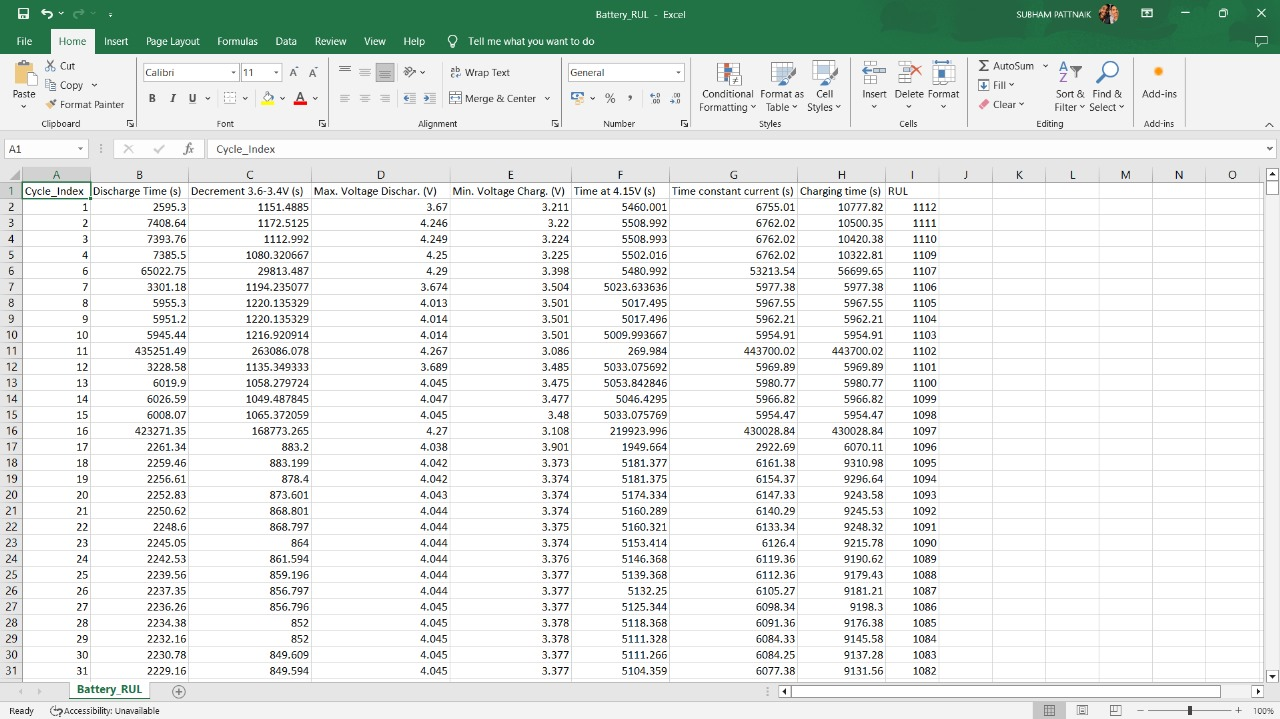
\includegraphics[width=0.9\textwidth]{datset.jpg} % Adjust the width as needed
    \caption{Battery Data Set}
    \label{fig:another}
\end{figure}

\section{Types of Battery Data for RUL Prediction}

When predicting how long a battery will last, known as its Remaining Useful Life (RUL), it's crucial to look at different types of data that tell us about the battery's health and performance. One key type of data is the charge and discharge cycles, which show how many times the battery has been used and recharged. This helps us understand how much wear and tear the battery has gone through. Another important data type is the voltage and current measurements during these cycles. These figures tell us if the battery is performing as expected or if it's starting to lose its ability to hold a charge. Temperature data is also vital because batteries can be sensitive to high or low temperatures, which can affect their performance and lifespan. By keeping an eye on these types of data, we can get a good idea of when a battery might need to be replaced before it fails unexpectedly.

\vspace{0.4in}
\textbf{Variables:}

\begin{itemize}
    \item \textbf{Cycle Index (Cycle):} 
    \begin{itemize}
        \item \textbf{Description:} Sequential number identifying each cycle of the battery operation.
        \item \textbf{Importance:} Helps track the chronological order of battery cycles, essential for time-series analysis and understanding degradation trends over time.
    \end{itemize}
    \item \textbf{F1: Discharge Time (s):} 
    \begin{itemize}
        \item \textbf{Description:} Duration of the discharge phase for each cycle in seconds.
        \item \textbf{Importance:} Indicates how long the battery was discharged during each cycle, influencing its wear and degradation rate.
    \end{itemize}
    \item \textbf{F2: Time at 4.15V (s):} 
    \begin{itemize}
        \item \textbf{Description:} Duration the battery spends at a voltage of 4.15V during charging, in seconds.
        \item \textbf{Importance:} Reflects the charging profile and helps in understanding the battery's state during specific voltage thresholds, impacting its longevity.
    \end{itemize}
    \item \textbf{F3: Time Constant Current (s):} 
    \begin{itemize}
        \item \textbf{Description:} Time spent at constant current during charging, in seconds.
        \item \textbf{Importance:} Provides insights into the charging behavior, affecting battery health and performance over multiple cycles.
    \end{itemize}
    \item \textbf{F4: Decrement 3.6-3.4V (s):} 
    \begin{itemize}
        \item \textbf{Description:} Time taken for the voltage to drop from 3.6V to 3.4V during discharge, in seconds.
        \item \textbf{Importance:} Indicates the discharge profile and helps in assessing the battery's capacity degradation over cycles.
    \end{itemize}
    \item \textbf{F5: Max. Voltage Discharge (V):} 
    \begin{itemize}
        \item \textbf{Description:} Maximum voltage recorded during the discharge phase of each cycle, in volts.
        \item \textbf{Importance:} Reflects the peak performance and capacity of the battery during discharge, crucial for RUL estimation.
    \end{itemize}
    \item \textbf{F6: Min. Voltage Charge (V):} 
    \begin{itemize}
        \item \textbf{Description:} Minimum voltage recorded during the charging phase of each cycle, in volts.
        \item \textbf{Importance:} Indicates the lowest point of the battery voltage during charging, influencing its charging efficiency and health.
    \end{itemize}
    \item \textbf{F7: Charging Time (s):} 
    \begin{itemize}
        \item \textbf{Description:} Total duration of the charging phase for each cycle, in seconds.
        \item \textbf{Importance:} Reflects the overall charging process, which affects the battery's degradation and lifespan.
    \end{itemize}
    \item \textbf{Total time (s):} 
    \begin{itemize}
        \item \textbf{Description:} Total accumulated time of battery operation up to the current cycle, in seconds.
        \item \textbf{Importance:} Provides a cumulative measure of the battery's usage history, aiding in understanding long-term degradation trends.
    \end{itemize}
    \item \textbf{RUL (Remaining Useful Life):} 
    \begin{itemize}
        \item \textbf{Description:} Target variable indicating the remaining cycles or time until the battery is considered no longer usable.
        \item \textbf{Importance:} This is the variable to be predicted using the other features. It directly measures the health and longevity of the battery based on historical data.
    \end{itemize}
\end{itemize}

\section{Importance of the Variables}

\begin{itemize}
    \item \textbf{Cycle Index:} Tracks the chronological order of cycles, essential for time-series analysis and understanding degradation trends.
    \item \textbf{Discharge Time (F1):} Indicates how long the battery is actively discharging, impacting its wear and degradation rate.
    \item \textbf{Time at 4.15V (F2):} Reflects charging profiles and states during specific voltage thresholds, influencing battery longevity.
    \item \textbf{Time Constant Current (F3):} Provides insights into charging behavior, affecting battery health and performance over cycles.
    \item \textbf{Decrement 3.6-3.4V (F4):} Indicates discharge profile and capacity degradation over cycles.
    \item \textbf{Max. Voltage Discharge (F5):} Reflects peak performance and capacity during discharge, crucial for RUL estimation.
    \item \textbf{Min. Voltage Charge (F6):} Indicates lowest voltage point during charging, affecting charging efficiency and battery health.
    \item \textbf{Charging Time (F7):} Reflects overall charging process, influencing degradation and lifespan.
    \item \textbf{Total time:} Cumulative measure of battery usage history, aiding in understanding long-term degradation trends.
    \item \textbf{RUL:} An objective variable indicating remaining service life, important for measuring battery health and estimating service life.
\end{itemize}

\section{Data Processing Technique}

To prepare this dataset for ML model training, several preprocessing steps would typically be applied:

\begin{itemize}
    \item \textbf{Data Cleaning:} Remove or impute missing values, correct erroneous data points, and handle outliers to ensure data quality.
    \item \textbf{Normalization:} Scale numerical features to a standard range (e.g., 0 to 1) to avoid dominance of certain features due to their magnitude.
    \item \textbf{Feature Engineering:} To enhance predictive power, create new features, or transform existing ones (e.g., calculate charge/discharge rates, derive cumulative degradation indicators).
    \item \textbf{Time Alignment:} Align time-series data to ensure consistency in timestamps and handle irregular sampling intervals.
    \item \textbf{Feature Selection:} Based on domain knowledge and statistical analysis, identify and select the most relevant features that significantly influence RUL prediction.
\end{itemize}

By leveraging these variables and applying robust data preprocessing techniques, ML models can effectively learn from historical battery data to predict Remaining Useful Life (RUL) accurately. This capability supports proactive maintenance strategies, optimizing battery performance, longevity, and cost-effectiveness in various applications.


\chapter{Implementation}
The implementation involves predicting the Remaining Useful Life (RUL) of the batteries using various machine learning models. The models were trained and evaluated using a dataset containing features related to battery performance and degradation.

\section{RUL and EDA Prediction}
In this section, we use various Python libraries to assist in the analysis and prediction of Remaining Useful Life (RUL). The libraries imported are as follows:
\begin{verbatim}
import pandas as pd 
import numpy as np 
import matplotlib.pyplot as plt 
import seaborn as sns 
import plotly as pl 
import warnings 
from pandas_profiling import ProfileReport 
from sklearn.model_selection import train_test_split 
from sklearn.preprocessing import RobustScaler 
from sklearn.model_selection import GridSearchCV 
from sklearn.linear_model import LinearRegression 
from sklearn.metrics import mean_squared_error 
from sklearn.tree import DecisionTreeRegressor 
from sklearn.ensemble import RandomForestRegressor 
from sklearn.pipeline import make_pipeline 
from sklearn.svm import SVR 
from sklearn.model_selection import cross_val_score 
from sklearn.metrics import classification_report, confusion_matrix 
from sklearn.neighbors import KNeighborsRegressor 
from sklearn.svm import SVR 
from sklearn.tree import plot_tree 
from sklearn.preprocessing import StandardScaler 
import seaborn as sns 
from sklearn.metrics import roc_curve, auc
\end{verbatim}
These are the various types of Python libraries imported for various purposes such as:
\begin{itemize}
    \item \texttt{pandas}: For data manipulation and analysis.
    \item \texttt{numpy}: For scientific computing and working with arrays.
    \item \texttt{matplotlib}: For data visualization.
    \item \texttt{seaborn}: For data visualization with a focus on statistical graphics.
    \item \texttt{plotly}: For interactive data visualization.
    \item \texttt{warnings}: For handling warnings.
    \item \texttt{pandas\_profiling}: For generating a report on the data.
    \item \texttt{train\_test\_split}: For splitting data into training and testing sets.
    \item \texttt{RobustScaler}: For scaling features.
    \item \texttt{GridSearchCV}: For performing grid search on hyperparameters.
\end{itemize}
\\
\noindent
\textbf{I/P} \\[-2.5em] % Reduced vertical space between heading and code

\begin{verbatim}
    from google.colab import files # Import the 'files' object
    from google.colab
\end{verbatim}
\\
This Command is used to import files from your local device \\
\\
\noindent
\textbf{I/P} \\[-2.5em] % Reduced vertical space between heading and code

\begin{verbatim}
    data = pd.read_csv("Battery_RUL.csv") 
\end{verbatim}
\\
pd.read\_csv() is a method provided by pandas to read data from a CSV file into a pandas DataFrame. Here, we are reading a CSV file named "Battery\_RUL.csv" using this method and storing the resulting DataFrame in a variable called data. This command assumes that the CSV file is in the same directory as our script. If the file is located elsewhere, you can specify the full path to the file instead of just the file name.
\newpage
\noindent
\textbf{I/P} \\[-1.5em] % Reduced vertical space between heading and code

\begin{verbatim}
    data.head() 
\end{verbatim}
\\
data.head() is a method to display the first few rows of the DataFrame data. By default, it 
displays the first five rows of the DataFrame, but we can specify the number of rows we want 
to display by passing an integer argument to the method. 
This method is useful for quickly inspecting the contents of our DataFrame and making sure 
that the data has been loaded correctly. It can also help us to identify any potential issues with 
our data such as missing values or incorrect data types.

\begin{table}[h!]
\centering
\caption{Battery Data}
\resizebox{\textwidth}{!}{%
\begin{tabular}{|c|c|c|c|c|c|c|c|c|}
\hline
\textbf{Cycle Index} & \textbf{Discharge Time (s)} & \textbf{Decrement} & \textbf{Max. Voltage (V)} & \textbf{Min. Voltage (V)} & \textbf{Time at 4.15V (s)} & \textbf{Time constant current (s)} & \textbf{Charging time (s)} & \textbf{RUL} \\
\hline
0 & 2595.30 & 3.6-3.4 & 1151.49 & 3.670 & 1112.99 & 5460.00 & 6.0 & 1080.32 \\
1 & 7408.64 & 4.0-3.8 & 1172.51 & 3.674 & 5508.99 & 10777.82 & 10500.35 & 10500.35 \\
2 & 7393.76 & 4.2-4.0 & 1190.11 & 3.680 & 5508.99 & 10322.81 & 10420.38 & 10322.81 \\
3 & 6.0 & 4.4-4.2 & 1200.50 & 3.690 & 5502.02 & 10420.38 & 10420.38 & 10420.38 \\
4 & 1080.32 & 4.6-4.4 & 1205.33 & 3.692 & 5480.99 & 10500.35 & 10322.81 & 10322.81 \\
\hline
\end{tabular}%
}
\label{tab:battery_data}
\end{table}
\\
\noindent
\textbf{I/P} \\[-1.5em] % Reduced vertical space between heading and code

\begin{verbatim}
    data.shape 
\end{verbatim}
\\
data.shape is a command that returns the dimensions of the DataFrame data. 
It returns a tuple of two elements where the first element is the number of rows in the DataFrame and the second element is the number of columns. 
\\
\\
\noindent
\textbf{O/P} \\[-1.5em] % Reduced vertical space between heading and code
\begin{verbatim}
    (15064, 9)
\end{verbatim}
\\
\\
\\
\noindent
\textbf{I/P} \\[-2.5em] % Reduced vertical space between heading and code
\\
\begin{verbatim}
def get_metadata(dataframe): 
    ''' 
    A function that fetches all the Metadata Information about
        the Dataframe 
    This function can be reused for all Pandas Dataframe 
    ''' 
        print("\nBASIC INFORMATION\n") 
        print(dataframe.info()) 
        print("=" * 100) 
        print("STATISTICAL INFORMATION") 
            display(dataframe.describe(include='all')) 
        print("=" * 100) 
        print("Dataframe Shape\n", dataframe.shape) 
        print("=" * 100) 
        print("Number of Duplicate Rows\n",
                dataframe.duplicated().sum()) 
        print("=" * 100) 
        print("NULL Values Check") 
        print(dataframe.isnull().sum()) 
        print("=" * 100) 
\end{verbatim}
\\
\noindent
This is a Python function called \texttt{get\_metadata} that takes a pandas DataFrame as an argument. 
The purpose of this function is to return various metadata information about the input DataFrame.

Here's a breakdown of what this function does:
\begin{itemize}
    \item The function first prints the string \texttt{"BASIC INFORMATION"} and then prints the result 
    of \texttt{dataframe.info()}. This method provides basic information about the DataFrame 
    such as the number of non-null values for each column, the data type of each column, 
    and the memory usage of the DataFrame.
    \item The function then prints a line of equal signs (=) to visually separate the output.
    \item Next, the function prints the string \texttt{"STATISTICAL INFORMATION"} and then uses 
    the \texttt{display()} method to print the result of\\ \texttt{dataframe.describe(include='all')}. This 
    method provides various statistical information about the DataFrame such as the 
    count, mean, standard deviation, minimum, and maximum values for each column.
    \item The function then prints another line of equal signs.
    \item Next, the function prints the string \texttt{"Dataframe Shape"} followed by the shape of the 
    DataFrame using the \texttt{shape} attribute of the DataFrame object.
    \item The function then prints another line of equal signs.
    \item Next, the function prints the string \texttt{"Number of Duplicate Rows"} followed by the 
    number of duplicate rows in the DataFrame using the \texttt{duplicated().sum()} method.
    \item The function then prints another line of equal signs.
    \item Finally, the function prints the string \texttt{"NULL Values Check"} followed by the number of 
    null values in each column using the \texttt{isnull().sum()} method.
\end{itemize}
\noindent
\textbf{I/P} \\[-1.5em] % Reduced vertical space between heading and code

\begin{verbatim}
    get_metadata(data)
\end{verbatim}
\\
\noindent
The command \texttt{get\_metadata(data)} will execute the \texttt{get\_metadata} function on the 
DataFrame \texttt{data}. 

This will print various metadata information about the DataFrame \texttt{data}, including basic 
information, statistical information, the shape of the DataFrame, the number of duplicate 
rows, and the number of null values in each column. 

This function can be useful for quickly getting an overview of the contents of a DataFrame and 
identifying any potential issues with the data.
\\
\\
\noindent
\textbf{BASIC INFORMATION}
\begin{adjustbox}{\textwidth}
\begin{verbatim}
<class 'pandas.core.frame.DataFrame'> 
RangeIndex: 15064 entries, 0 to 15063 
Data columns (total 9 columns): 
 #   Column                     Non-Null Count  Dtype   
 ---  ------                     --------------  -----   
 0   Cycle_Index                15064 non-null  float64 
 1   Discharge Time (s)         15064 non-null  float64 
 2   Decrement 3.6-3.4V (s)     15064 non-null  float64 
 3   Max. Voltage Dischar. (V)  15064 non-null  float64 
 4   Min. Voltage Charg. (V)    15064 non-null  float64 
 5   Time at 4.15V (s)          15064 non-null  float64 
 6   Time constant current (s)  15064 non-null  float64 
 7   Charging time (s)          15064 non-null  float64 
 8   RUL                        15064 non-null  int64   
dtypes: float64(8), int64(1) 
memory usage: 1.0 MB 
\end{verbatim}
\end{adjustbox}
\vspace{0.35in}
\noindent
\textbf{STATISTICAL INFORMATION}

\begin{table}[ht]
\centering
\resizebox{\textwidth}{!}{ % Resize the table to fit the text width
\begin{tabular}{lccccccccc}
\toprule
 & \textbf{Cycle\_Index} & \textbf{Discharge Time (s)} & \textbf{Decrement 3.6-3.4V (s)} & \textbf{Max. Voltage Dischar. (V)} & \textbf{Min. Voltage Charg. (V)} & \textbf{Time at 4.15V (s)} & \textbf{Time constant current (s)} & \textbf{Charging time (s)} & \textbf{RUL} \\
\midrule
Count & 15064 & 15064 & 15064 & 15064 & 15064 & 15064 & 15064 & 15064 & 15064 \\
Mean & 556.15500 & 4581.27396 & 1239.78467 & 3.908176 & 3.577904 & 3768.33617 & 5461.26670 & 10066.49620 & 554.19417 \\
Std & 322.37848 & 33144.01207 & 15039.58927 & 0.091003 & 0.123695 & 9129.55248 & 25155.84520 & 26415.35412 & 322.43451 \\
Min & 1.00000 & 8.69000 & 3976.90900 & 3.04300 & 3.02200 & 113.58400 & 5.98000 & 5.98000 & 0.00000 \\
25\% & 271.00000 & 1169.31000 & 319.60000 & 3.84600 & 3.48800 & 1828.84179 & 2564.31000 & 7841.92250 & 277.00000 \\
50\% & 560.00000 & 1557.25000 & 439.23947 & 3.90600 & 3.57400 & 2930.20350 & 3824.26000 & 8320.41500 & 551.00000 \\
75\% & 833.00000 & 1908.00000 & 600.00000 & 3.97200 & 3.66300 & 4088.32650 & 5012.35000 & 8763.28500 & 839.00000 \\
Max & 1134.00000 & 958320.37000 & 406703.76800 & 4.36300 & 4.37900 & 245101.11700 & 880728.10000 & 880728.10000 & 1133.00000 \\
\bottomrule
\end{tabular}
}
\end{table}

\noindent
\textbf{Dataframe Shape}

\begin{adjustbox}
\footnotesize
\begin{verbatim}
(15064, 9)
\end{verbatim}
\end{adjustbox}

\newpage
\noindent
\textbf{Number of Duplicate Rows}

\begin{adjustbox}
\footnotesize
\begin{verbatim}
0
\end{verbatim}
\end{adjustbox}

\noindent
\textbf{NULL Values Check}

\begin{adjustbox}
\footnotesize
\begin{verbatim}
Cycle_Index                  0 
Discharge Time (s)           0 
Decrement 3.6-3.4V (s)       0 
Max. Voltage Dischar. (V)    0 
Min. Voltage Charg. (V)      0 
Time at 4.15V (s)            0 
Time constant current (s)    0 
Charging time (s)            0 
RUL                          0 
dtype: int64 
\end{verbatim}
\end{adjustbox}
\\
\noindent
\textbf{I/P} \\[-1.5em] % Reduced vertical space between heading and code

\begin{verbatim}
    profile = ProfileReport(data) 
    profile  
\end{verbatim}
\\
The command \texttt{profile = ProfileReport(data)} will create a \texttt{ProfileReport} object for the DataFrame \texttt{data} using the pandas-profiling library. This object will contain a comprehensive report of various statistics and visualizations for the DataFrame, including basic information, variable types, descriptive statistics, correlations, 
missing values, and much more. You can then view the report by simply calling the \texttt{profile} object.\\
\\
\noindent
\textbf{I/P} \\[-1.5em] % Reduced vertical space between heading and code

\begin{verbatim}
    profile = ProfileReport(data) 
    profile  
\end{verbatim}
\\
The command \texttt{profile = ProfileReport(data)} will create a \texttt{ProfileReport} object for the DataFrame \texttt{data} using the pandas-profiling library. This object will contain a comprehensive report of various statistics and visualizations for the DataFrame, including basic information, variable types, descriptive statistics, correlations, missing values, and much more. You can then view the report by simply calling the \texttt{profile} object.
\newpage
\noindent
\textbf{O/P} \\[-1.5em] % Reduced vertical space between heading and code

\begin{figure}[h!]
    \centering
    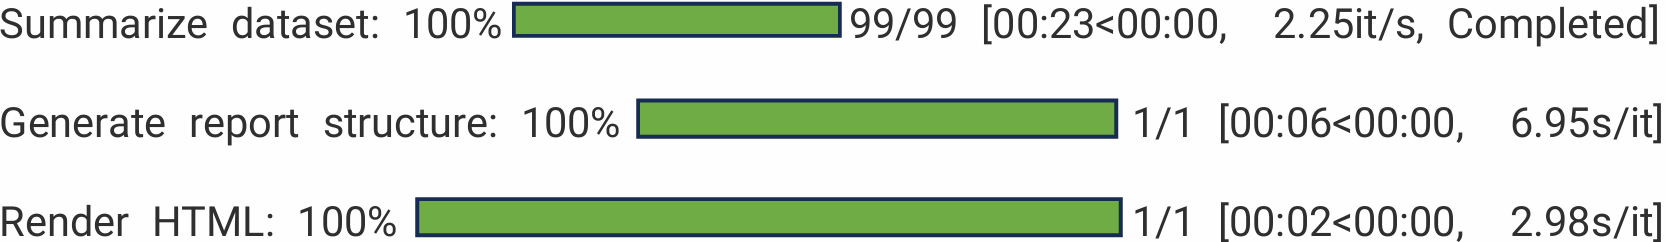
\includegraphics[width=\textwidth]{grapph.png}
\end{figure}
\begin{figure}[h!]
    \centering
    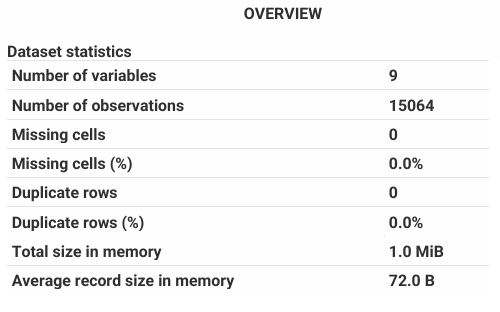
\includegraphics[width=1\textwidth]{overview.png} 
    \label{fig:another}
\end{figure}

\section{Exploratory Data Analysis (EDA)}
Exploratory Data Analysis (EDA) was conducted to understand the relationships between different features and the target variable (RUL). Various Python libraries such as matplotlib and seaborn were utilized to create visualizations. The following visualizations and analyses were performed:\\
\\
\noindent
\textbf{I/P} \\[-2.5em] % Reduced vertical space between heading and code
\begin{verbatim}
    plt.title('RUL, Remaining Useful Time Histogram') 
    sns.histplot(data.RUL, kde=True) 
    plt.show()   
\end{verbatim}

\subsection{Histogram of RUL}
The code provided uses Python libraries \texttt{matplotlib} and \texttt{seaborn} to create a histogram of the \texttt{RUL} (Remaining Useful Life) column in the \texttt{data} DataFrame. Here’s what each line of code does:

\begin{itemize}
    \item \texttt{plt.title('RUL, Remaining Useful Time Histogram')}: Sets the title of the plot to "RUL, Remaining Useful Time Histogram" using \texttt{plt.title()} from \texttt{matplotlib.pyplot}.
    \item \texttt{sns.histplot(data.RUL, kde=True)}: Creates a histogram of the \texttt{RUL} column in the \texttt{data} using \texttt{sns.histplot()} from \texttt{seaborn}. The argument \texttt{kde=True} adds a kernel density estimate (KDE) plot to the histogram.
    \item \texttt{plt.show()}: Displays the plot using \texttt{plt.show()} from \texttt{matplotlib.pyplot}.
\end{itemize}
Overall, this code will create a histogram with a KDE plot overlaid on top to show the distribution of the \texttt{RUL} column in the \texttt{data} DataFrame.
\begin{figure}[H]
    \centering
    \textbf{I/P} \\[-2.5em]
    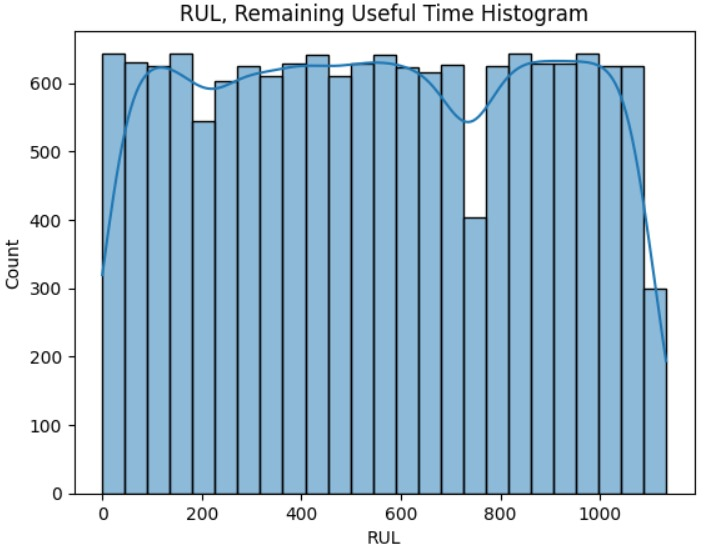
\includegraphics[width=0.8\textwidth]{rul_histogram.jpg}
    \caption{RUL Histogram}
    \label{fig:rul_histogram}
\end{figure}

\subsection{Correlation Heatmap}\\
\\
\noindent
\textbf{I/P} \\[-1.5em] % Reduced vertical space between heading and code
\begin{verbatim}
    plt.figure(figsize = (15,8)) 
    sns.heatmap(data.corr(),annot=True, cbar=False, 
                    cmap='Blues', fmt='.1f')  
\end{verbatim}
The code provided uses Python libraries \texttt{matplotlib} and \texttt{seaborn} to create a correlation heatmap for the \texttt{data} DataFrame. Here’s what each line of code does:
\begin{itemize}
    \item \texttt{plt.figure(figsize = (15,8))}: Sets the size of the plot to 15 inches wide and 8 inches tall using \texttt{plt.figure()} from \texttt{matplotlib.pyplot}.
    \item \texttt{sns.heatmap(data.corr(), annot=True, cbar=False, cmap='Blues', fmt='.1f')}: Creates a correlation heatmap for the \texttt{data} DataFrame using \texttt{sns.heatmap()} from \texttt{seaborn}. The argument \texttt{data.corr()} calculates the correlation between all pairs of columns in the DataFrame.
\end{itemize}
Overall, this code will create a heatmap to visualize the correlation between different features in the \texttt{data} DataFrame.\\
\newpage
\noindent
\textbf{I/P} \\[-2.5em] % Reduced vertical space between heading and code
\begin{verbatim}
    data=data.drop(['Cycle_Index',
                    'Discharge Time (s)', 
                    'Decrement 3.6-3.4V (s)', 
                    'Time constant current (s)',
                    'Charging time (s)'],axis=1)  
\end{verbatim}
\begin{figure}[H]
    \centering
    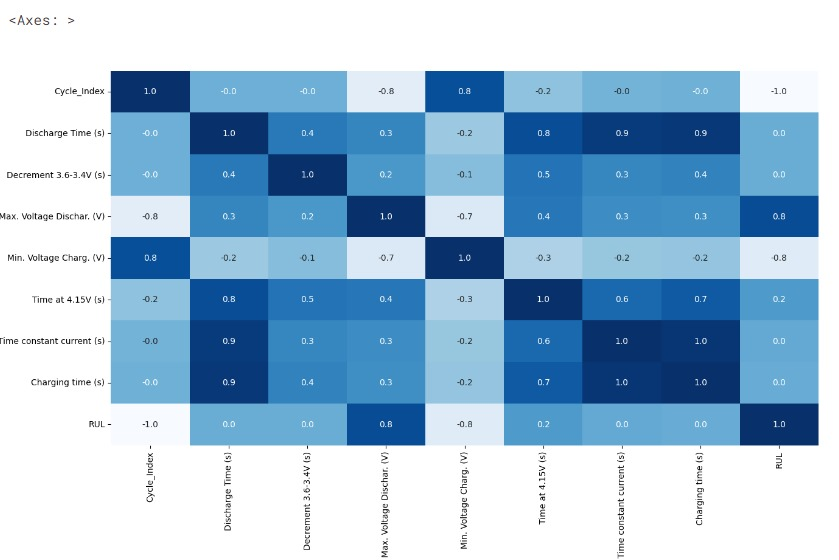
\includegraphics[width=0.8\textwidth]{correlation_heatmap.jpg}
    \caption{Correlation Heatmap for the Data DataFrame}
    \label{fig:correlation_heatmap}
\end{figure}

\subsection{Scatter Plot: Max Voltage Discharge vs. RUL}
\\
\noindent
\textbf{I/P} \\[-2.5em] % Reduced vertical space between heading and code
\begin{verbatim}
    plt.figure(figsize=(10, 6)) 
    plt.scatter(data['Max. Voltage Dischar. (V)'], 
                        data['RUL'], alpha=0.5) 
    plt.title('Scatter Plot: Max. Voltage 
                    Discharge vs. Remaining Useful Lifetime') 
    plt.xlabel('Max. Voltage Dischar. (V)') 
    plt.ylabel('Remaining Useful Lifetime (RUL)') 
    plt.grid(True) 
    plt.show()    
\end{verbatim}
The code provided creates a scatter plot of the Max. Voltage Discharge (V) column against the RUL column in the \texttt{data} DataFrame. Here’s what each line of code does:
\begin{itemize}
    \item \texttt{plt.figure(figsize=(10, 6))}: Sets the size of the plot to 10 inches wide and 6 inches tall.
    \item \texttt{plt.scatter(data['Max. Voltage Dischar. (V)'], data['RUL'], alpha=0.5)}: Creates a scatter plot with the Max. Voltage Discharge (V) on the x-axis and RUL on the y-axis. The \texttt{alpha=0.5} argument sets the transparency of the points.
    \item \texttt{plt.title('Scatter Plot: Max. Voltage Discharge vs. Remaining Useful Lifetime')}: Sets the title of the plot.
    \item \texttt{plt.xlabel('Max. Voltage Dischar. (V)')}: Sets the x-axis label.
    \item \texttt{plt.ylabel('Remaining Useful Lifetime (RUL)')}: Sets the y-axis label.
    \item \texttt{plt.grid(True)}: Adds a grid to the plot.
    \item \texttt{plt.show()}: Displays the plot.
\end{itemize}
This code will create a scatter plot to visualize the relationship between Max. Voltage Discharge (V) and RUL.
\begin{figure}[H]
    \centering
    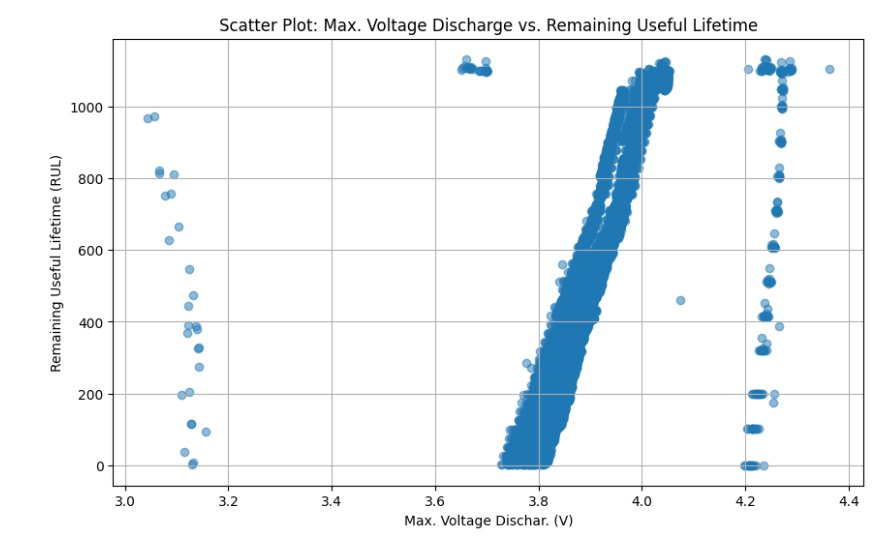
\includegraphics[width=0.7\textwidth]{scatter_plot_max_voltage_vs_rul.jpg}
    \caption{Scatter Plot: Max Voltage Discharge Vs RUL}
    \label{fig:scatter_plot_max_voltage_vs_rul}
\end{figure}

\subsection{Scatter Plot: Min Voltage Charge vs. RUL}
Similarly, the code provided creates a scatter plot of the Min. Voltage Charge (V) column against the RUL column in the data DataFrame. Here’s what each line of code does:
\begin{itemize}
    \item \texttt{plt.figure(figsize=(10, 6))}: Sets the size of the plot to 10 inches wide and 6 inches tall.
    \item \texttt{plt.scatter(data['Min. Voltage Charg. (V)'], data['RUL'], alpha=0.5)}: Creates a scatter plot with the Min. Voltage Charge (V) on the x-axis and RUL on the y-axis. The \texttt{alpha=0.5} argument sets the transparency of the points.
    \item \texttt{plt.title('Scatter Plot: Min. Voltage Charge vs. Remaining Useful Lifetime')}: Sets the title of the plot.
    \item \texttt{plt.xlabel('Min. Voltage Charg. (V)')}: Sets the x-axis label.
    \item \texttt{plt.ylabel('Remaining Useful Lifetime (RUL)')}: Sets the y-axis label.
    \item \texttt{plt.grid(True)}: Adds a grid to the plot.
    \item \texttt{plt.show()}: Displays the plot.
\end{itemize}
This code will create a scatter plot to visualize the relationship between Min. Voltage Charge (V) and RUL.\\
\noindent
\textbf{I/P} \\[-2.5em] % Reduced vertical space between heading and code
\begin{verbatim}
    plt.figure(figsize=(10, 6))  
    plt.scatter(data['Min. Voltage Charg. (V)'],
                        data['RUL'], alpha=0.5) 
    plt.title('Scatter Plot: Min. Voltage 
                    Charge vs. Remaining Useful Lifetime') 
    plt.xlabel('Min. Voltage Charg. (V)')  
    plt.ylabel('Remaining Useful Lifetime (RUL)') 
    plt.grid(True) 
    plt.show()    
\end{verbatim}
\newpage
\begin{figure}[H]
    \centering
    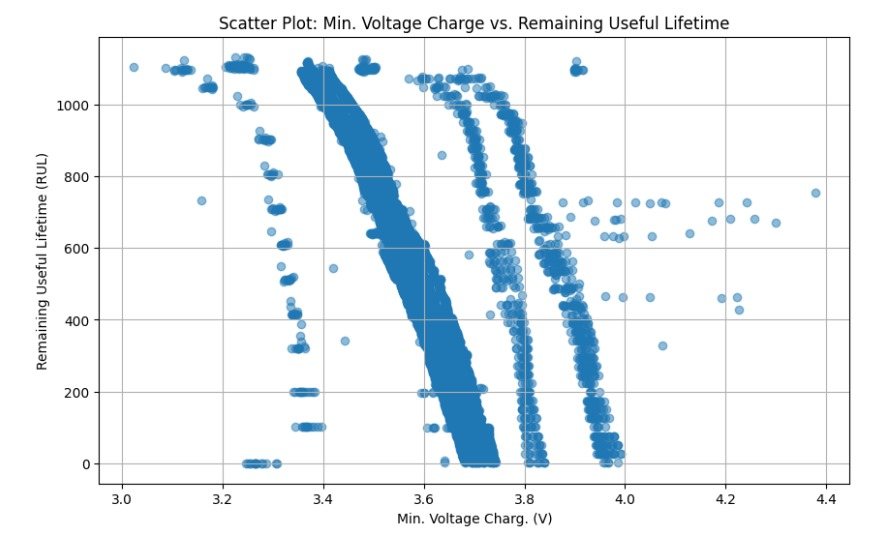
\includegraphics[width=0.7\textwidth]{scatter_plot_min_voltage_vs_rul.jpg}
    \caption{Scatter Plot: Min Voltage Charge Vs RUL}
    \label{fig:scatter_plot_min_voltage_vs_rul}
\end{figure}

\subsection{Scatter Plot: Time at 4.15V Vs RUL}
\noindent
\textbf{I/P} \\[-2.5em] % Reduced vertical space between heading and code
\begin{verbatim}
    plt.figure(figsize=(10, 6)) 
    plt.scatter(data['Time at 4.15V (s)'],
                            data['RUL'], alpha=0.5) 
    plt.title('Scatter Plot: Time at 4.15V vs. Remaining 
                                Useful Lifetime') 
    plt.xlabel('Time at 4.15V (s)') 
    plt.ylabel('Remaining Useful Lifetime (RUL)') 
    plt.grid(True) 
    plt.show()    
\end{verbatim}
\begin{figure}[H]
    \centering
    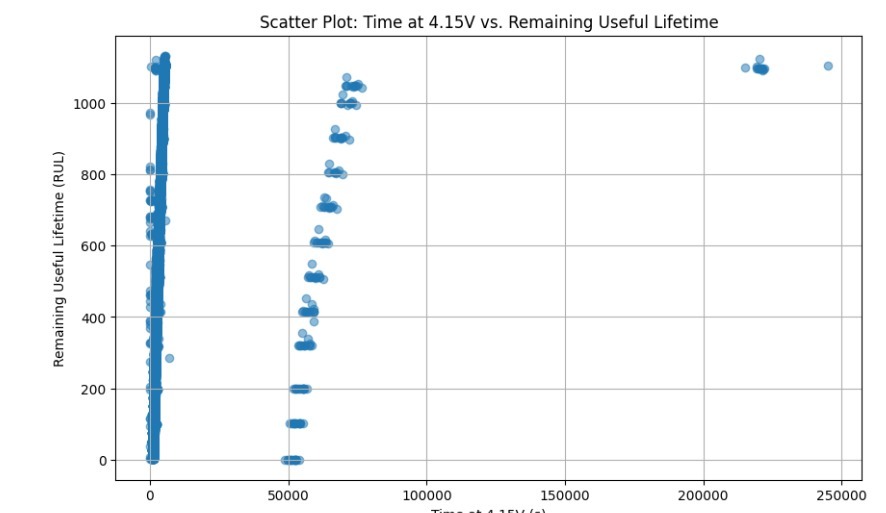
\includegraphics[width=0.7\textwidth]{scatter_plot.jpg}
    \caption{Scatter Plot: Time at 4.15V Vs RUL}
    \label{fig:scatter_plot_min_voltage_vs_rul}
\end{figure}

\section{Mathmetical method's }
\subsection{Calculation of R\textsuperscript{2} Score}
$R^2$ (R-squared) is a metric used to evaluate the performance of linear regression models. It essentially tells you how well the regression line fits the actual data points.

\subsubsection{Formula}
The $R^2$ value is calculated using the following formula:
\begin{equation*}
    R^2 = 1 - \frac{SSR}{SST}
\end{equation*}

Where:
\begin{itemize}
    \item $R^2$: The R-squared value (between 0 and 1)
    \item SSR (Sum of Squared Residuals): The total squared difference between the predicted values by the model and the actual values.
    \item SST (Total Sum of Squares): The total squared difference between the actual values and the mean of the actual values.
\end{itemize}

\subsubsection{Interpretation}
\begin{itemize}
    \item A higher $R^2$ value (closer to 1) indicates a better fit. The model explains a larger proportion of the variance in the data.
    \item An $R^2$ of 1 means a perfect fit, where the regression line exactly matches all the data points.
    \item An $R^2$ of 0 means the model doesn't explain any of the variance in the data, and the regression line is just a horizontal line at the mean of the actual values.
\end{itemize}

\subsubsection{Steps to Calculate $R^2$}
\begin{enumerate}
    \item Calculate the mean of the actual values ($\bar{y}$):
    \begin{equation*}
        \bar{y} = \frac{1}{n} \sum_{i=1}^n y_i
    \end{equation*}
    
    \item For each data point:
    \begin{itemize}
        \item Calculate the difference between the actual value ($y_i$) and the mean ($\bar{y}$). Square this difference:
        \begin{equation*}
            (y_i - \bar{y})^2
        \end{equation*}
    \end{itemize}
    
    \item Sum the squared differences from step 2. This is SST:
    \begin{equation*}
        SST = \sum_{i=1}^n (y_i - \bar{y})^2
    \end{equation*}
    
    \item For each data point:
    \begin{itemize}
        \item Calculate the difference between the predicted value ($\hat{y}_i$) by the model and the actual value ($y_i$). Square this difference:
        \begin{equation*}
            (\hat{y}_i - y_i)^2
        \end{equation*}
    \end{itemize}
    
    \item Sum the squared differences from step 4. This is SSR:
    \begin{equation*}
        SSR = \sum_{i=1}^n (\hat{y}_i - y_i)^2
    \end{equation*}
    
    \item Apply the formula:
    \begin{equation*}
        R^2 = 1 - \frac{SSR}{SST}
    \end{equation*}
\end{enumerate}

\subsection{CALCULATION OF ROOT MEAN SQUARE}
The Root Mean Square (RMS) can be calculated for a set of numbers or a continuous function. Here, we will focus on calculating it for a set of numbers.

\subsubsection{Formula}
The RMS value is calculated using the following formula:
\begin{equation*}
    \text{RMS} = \sqrt{\frac{x_1^2 + x_2^2 + \cdots + x_n^2}{N}}
\end{equation*}

Where:
\begin{itemize}
    \item \text{RMS}: The Root Mean Square value
    \item $x_1$ to $x_n$: The individual numbers in your data set
    \item $N$: The total number of numbers in your data set
\end{itemize}

\subsubsection{Steps to Calculate RMS}
\begin{enumerate}
    \item Square each number in your data set. This means multiplying each number by itself:
    \begin{equation*}
        x_i^2
    \end{equation*}
    
    \item Add up the squared values from step 1:
    \begin{equation*}
        \text{Sum} = x_1^2 + x_2^2 + \cdots + x_n^2
    \end{equation*}
    
    \item Divide the sum from step 2 by the total number of numbers ($N$) in your data set. This gives you the average of the squared values:
    \begin{equation*}
        \text{Average} = \frac{\text{Sum}}{N}
    \end{equation*}
    
    \item Take the square root of the result from step 3. This is the Root Mean Square (RMS) of your data set:
    \begin{equation*}
        \text{RMS} = \sqrt{\text{Average}}
    \end{equation*}
\end{enumerate}

\subsection{CALCULATION OF MEAN SQUARED ERROR}
Mean Squared Error (MSE) is a metric used to evaluate how well predictions from a model match the actual values. It provides a measure of the average squared difference between predicted and actual values.

\subsubsection{Formula}
The MSE value is calculated using the following formula:
\begin{equation*}
    \text{MSE} = \frac{1}{n} \sum_{i=1}^{n} (y_i - \hat{y}_i)^2
\end{equation*}

Where:
\begin{itemize}
    \item \text{MSE}: The Mean Squared Error value
    \item $\sum$: Summation symbol (indicates summing over all data points)
    \item $y_i$: The actual value for the $i$-th data point
    \item $\hat{y}_i$: The predicted value for the $i$-th data point by the model
    \item $n$: The total number of data points
\end{itemize}

\subsubsection{Steps to Calculate MSE}
\begin{enumerate}
    \item For each data point:
    \begin{itemize}
        \item Calculate the difference between the actual value ($y_i$) and the predicted value ($\hat{y}_i$) by the model:
        \begin{equation*}
            d_i = y_i - \hat{y}_i
        \end{equation*}
        \item Square this difference:
        \begin{equation*}
            (d_i)^2
        \end{equation*}
    \end{itemize}
    
    \item Sum the squared differences from step 1 for all data points:
    \begin{equation*}
        \text{Sum} = \sum_{i=1}^{n} (y_i - \hat{y}_i)^2
    \end{equation*}
    
    \item Divide the sum by the total number of data points ($n$). This gives you the average squared difference between predictions and actual values:
    \begin{equation**}
        \text{MSE} = \frac{\text{Sum}}{n}
    \end{equation**}
\end{enumerate}

\section{Modelling and Prediction}
The code provided is creating a feature matrix \texttt{X} and target vector \texttt{y} from the \texttt{data} DataFrame, where \texttt{X} contains all columns except for the \texttt{RUL} column and \texttt{y} contains only the \texttt{RUL} column. Here’s what each line of code does:

\begin{itemize}
    \item \texttt{X = data.drop(['RUL'], axis=1)}: Creates the feature matrix \texttt{X} by dropping the \texttt{RUL} column from the \texttt{data} DataFrame using \texttt{drop()} with \texttt{axis=1}.
    \item \texttt{y = data['RUL']}: Creates the target vector \texttt{y} by selecting only the \texttt{RUL} column from the \texttt{data} DataFrame.
\end{itemize}

Overall, this code will separate the features and target variable from the \texttt{data} DataFrame, which can be used for machine learning modeling or other analysis.\\
\\
\noindent
\textbf{I/P} \\[-1.5em]
\begin{verbatim}
    X = data.drop(['RUL'], axis=1)
    y = data['RUL']
\end{verbatim}
\noindent
\\
\textbf{I/P} \\[-1.5em] % Reduced vertical space between heading and code
\begin{verbatim}
    X_train, X_test, y_train, y_test = train_test_split
    (X, y, test_size=0.33, random_state=2023, shuffle=True)
\end{verbatim}
\newpage
\noindent
\textbf{I/P} \\[-1.5em]
\begin{verbatim}
class Pipeline:
    def __init__(self, scalar):
        self.scalar = scalar

    def fit(self, X, y):
        X = self.scalar.fit_transform(X)
        return X, y

    def transform(self, X, y):
        X = self.scalar.transform(X)
        return X, y
\end{verbatim}

The code provided defines a custom \texttt{Pipeline} class with methods for fitting and transforming data.

This class can be used to standardize or normalize the feature matrix \texttt{X} while leaving the target vector \texttt{y} unchanged.

\subsection{Linear Regression}
\noindent
\textbf{I/P} \\[-1.5em] 
\begin{verbatim}
    # Fit the model to the training data
        linear_regression.fit(X_train, y_train)

    # Make predictions on the training set
        y_train_pred = linear_regression.predict(X_train)

    # Make predictions on the test set
        y_test_pred = linear_regression.predict(X_test)

    # Evaluate the performance on the training set
        train_score = linear_regression.score(X_train, y_train)
        print("Score on Training Set: {:.2%}".format(train_score))

    # Calculate and print the R^2 score on the test set
        test_score = linear_regression.score(X_test, y_test)
        print("Score on Test Set: {:.2%}".format(test_score))
\end{verbatim}
\\
\noindent
\textbf{O/P} \\[-2.5em]
\begin{verbatim}
    Score on Training Set: 72.38% 
    Score on Test Set: 75.64% 
\end{verbatim}

\subsection{K-Nearest Neighbors}
\noindent
\textbf{I/P} \\[-1.5em] 
\begin{verbatim}
    # Fit the model to the training data
        knn.fit(X_train, y_train)

    # Make predictions on the training set
        y_train_pred = knn.predict(X_train)

    model = KNeighborsRegressor(n_neighbors=3).fit(X_train,y_train) 
    
    # Make predictions on the test set
        y_test_pred = knn.predict(X_test)
        y_predictions = model.predict(X_test)

    # Calculate and print the RMSE on the test set
        rmse = np.sqrt(mean_squared_error(y_test, y_test_pred))
        print('training score: '+ "{:.2%}".format
        (model.score(X_train, y_train))) 
        print('test score: '+ "{:.2%}".format(model.score(X_test,y_test))) 
        print('Root Mean Squared Error: '+ "{:.2f}".format
        (mean_squared_error(y_test,y_predictions,squared=False))) 
\end{verbatim}
\\
\noindent
\textbf{O/P} \\[-1.5em]
\begin{verbatim}
    Score on Training Set: 72.38% 
    Score on Test Set: 75.64% 
    Root Mean Squared Error: 29.95 
\end{verbatim}

\subsection{Support Vector Machine}
\noindent
\textbf{I/P} \\[-1.5em]
\begin{verbatim}
    svm_regressor = SVR(kernel='linear', C=1.0) 
 
    # Fit the model to the training data 
        svm_regressor.fit(X_train, y_train) 
 
    # Make predictions on the testing set 
        y_pred = svm_regressor.predict(X_test) 
 
    # Evaluate the model using Mean Squared Error (MSE) 
        mse = mean_squared_error(y_test, y_pred) 
        print(f'Mean Squared Error: {mse}') 
 
    # Evaluate the performance on the training set 
        train_score = svm_regressor.score(X_train, y_train) 
        print("Score on Training Set: {:.2%}".format(train_score)) 
 
    # Calculate and print the R^2 score on the test set 
        test_score = svm_regressor.score(X_test, y_test) 
        print("Score on Test Set: {:.2%}".format(test_score)) 
 
    # Visualize the predicted vs actual values 
    # plt.scatter(y_test, y_pred) 
    # plt.xlabel('Actual Values') 
    # plt.ylabel('Predicted Values') 
\end{verbatim}
\\
\noindent
\textbf{O/P} \\[-1.5em]
\begin{verbatim}
    Mean Squared Error: 28214.572819922752 
    Score on Training Set: 66.07% 
    Score on Test Set: 72.72%  
\end{verbatim}

\subsection{Decision Tree}
\noindent
\textbf{I/P} \\[-1.5em]
\begin{verbatim}
    # Create a decision tree regressor model 
        decision_tree = DecisionTreeRegressor() 
 
    # Define the hyperparameter grid 
        param_grid = { 
            'max_depth': [None, 5, 10, 15], 
            'min_samples_split': [2, 5, 10], 
            'min_samples_leaf': [1, 2, 4] 
        } 
 
    # Create the GridSearchCV object 
        grid_search = GridSearchCV(estimator=decision_tree,
                        param_grid=param_grid,
                        scoring='neg_mean_squared_error',
                        cv=5) 
 
    # Fit the model to the training data 
        grid_search.fit(X_train, y_train) 
 
    # Print the best parameters found by the grid search 
        print("Best Parameters: ", grid_search.best_params_) 
 
    # Get the best model 
        best_model1 = grid_search.best_estimator_ 
 
    # Make predictions on the test set 
        y_pred = best_model1.predict(X_test) 
 
    # Evaluate the performance of the best model 
        mse = mean_squared_error(y_test, y_pred) 
        print("Mean Squared Error on Test Set: ", mse) 
 
    train_score = best_model1.score(X_train, y_train) 
    print("Score on Training Set: {:.2%}".format(train_score)) 
\end{verbatim}
\\
\noindent
\textbf{O/P} \\[-1.5em]
\begin{verbatim}
    Best Parameters:  {'max_depth': None,
        'min_samples_leaf': 4, 'min_samples_split': 5} 
    Mean Squared Error on Test Set:  1390.199771972764 
    Score on Training Set: 99.56% 
    Score on Test Set: 98.66%  
\end{verbatim}
\begin{figure}[h!]{0.45\textwidth}
        \centering
        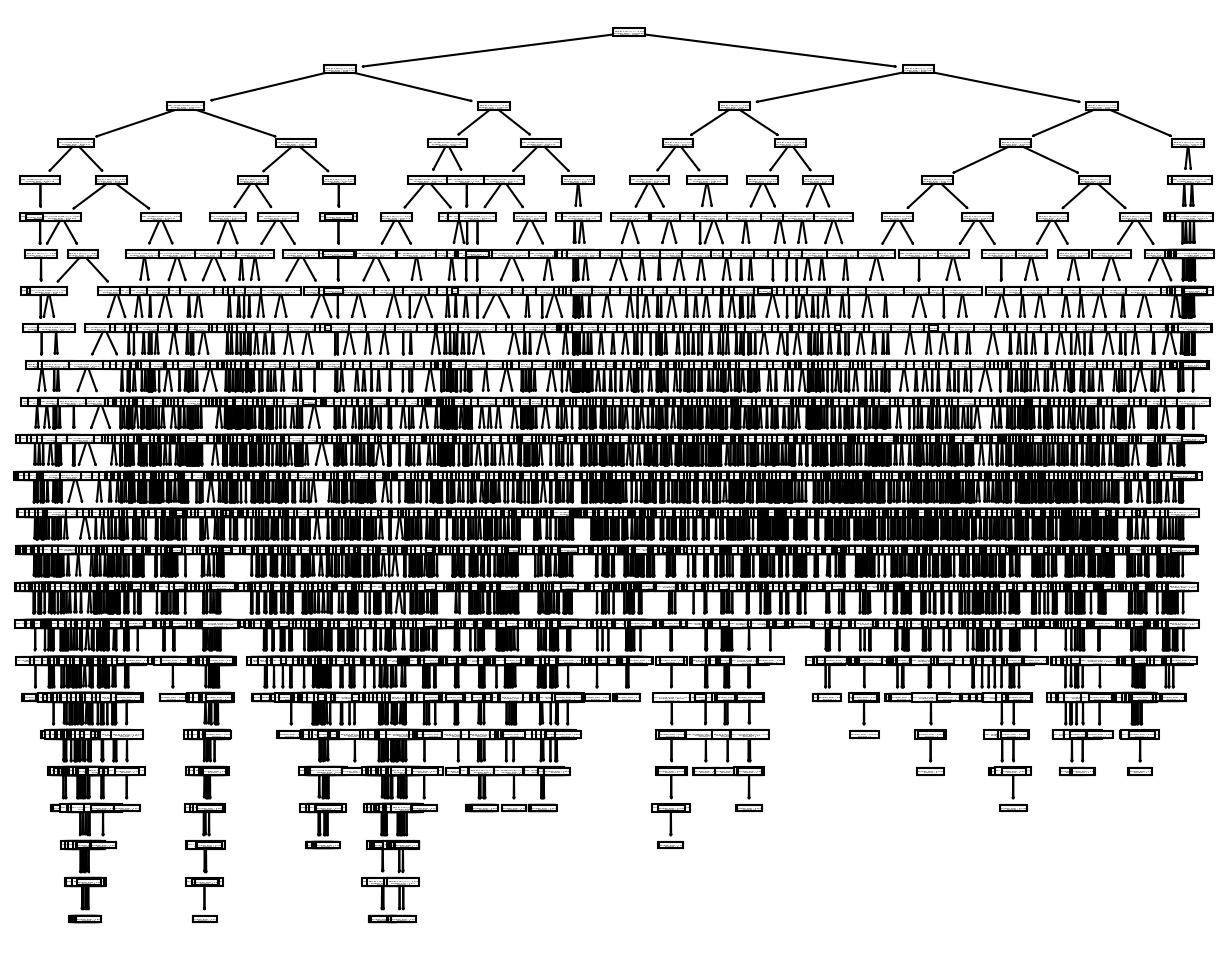
\includegraphics[width=\textwidth]{00000.jpg}
        \caption{1 Decision Tree Ploting }
        \label{fig:another2}
\end{figure}
\newpage
\subsection{Random Forest}
\noindent
\textbf{I/P} \\[-1.5em]
\begin{verbatim}
    random_forest = RandomForestRegressor() 
 
    # Define the hyperparameter grid 
        param_grid = {'n_estimators': [50, 100, 150], 
            'max_depth': [None, 5, 10, 15], 
            'min_samples_split': [2, 5, 10], 
            'min_samples_leaf': [1, 2, 4] } 
 
    # Create the GridSearchCV object 
    grid_search = GridSearchCV(estimator=random_forest,
                            param_grid=param_grid,
                            scoring='r2', cv=5) 
 
    # Fit the model to the training data 
    grid_search.fit(X_train, y_train) 
 
    # Print the best parameters found by the grid search 
    print("Best Parameters: ", grid_search.best_params_) 
 
    # Get the best model 
    best_model = grid_search.best_estimator_ 
 
    # Calculate and print the R^2 score on the training set 
    train_score = best_model.score(X_train, y_train) 
    print("R^2 Score on Training Set: {:.2%}".format(train_score)) 
 
    # Calculate and print the R^2 score on the test set 
    test_score = best_model.score(X_test, y_test) 
    print("R^2 Score on Test Set: {:.2%}".format(test_score)) 
\end{verbatim}
\\
\noindent
\textbf{O/P} \\[-1.5em]
\begin{verbatim}
    Best Parameters:  {'max_depth': None, 'min_samples_leaf': 1,
                        'min_samples_split': 2,
                        'n_estimators': 150} 
    R^2 Score on Training Set: 99.86% 
    R^2 Score on Test Set: 99.16%   
\end{verbatim}

\section{Best Model}
\noindent
\textbf{I/P} \\[-1.5em]
\begin{verbatim}
    def find_best_model(X, y):
        algorithms = {
            'Linear Regression': LinearRegression(),
            'Decision Tree': DecisionTreeRegressor(),
            'Random Forest': RandomForestRegressor(),
            'Support Vector Machine': make_pipeline(RobustScaler(), SVR()) }

    best_model_name = None
    best_score = float('-inf')

    for name, model in algorithms.items():
        # Using cross_val_score for simplicity
        scores = cross_val_score(model, X, y, cv=5, scoring='r2') 

        # Take the mean of cross-validation scores as the 
                            performance metric
        mean_score = scores.mean()

        print(f"{name} - R^2 Score: {mean_score:.4f}")

        # Update the best model if the current one has a higher score
        if mean_score > best_score:
            best_score = mean_score
            best_model_name = name

    print(f"\nBest Model: {best_model_name} with 
                                R^2 Score: {best_score:.4f}")

    # Assuming X is your feature matrix and y is your target variable
    # Replace X and y with your actual feature matrix 
    and target variable find_best_model(X, y)
\end{verbatim}
\begin{verbatim}
O/P
    Linear Regression - R^2 Score: 0.7156
    Decision Tree - R^2 Score: 0.9473
    Random Forest - R^2 Score: 0.9608
    Support Vector Machine - R^2 Score: 0.9190

    Best Model: Random Forest with R^2 Score: 0.9608
\end{verbatim}

